\clearpage
\section{Hardware}\label{sec:Hardware}
In diesem Kapitel wird die Hardware vom \textit{Gateway Interface System}, dem \textit{Universal Peripheral Node}, dem \textit{Energy Harvesting System} und dem \textit{Power Storage System} beschrieben. 


\subsection{Bluetooth Mesh Node (BMN)}\label{subsec:BMN}
Im Bluetooth Mesh Protokoll gibt es zwei verschiedene  Geräte, ein \textit{"'unprovisioned device"'} und einen \textit{"'node"'}. Das \textit{"'unprovisioned device"'}  ist ein Teilnehmer, der für das Mesh Netzwerk unbekannt ist und deshalb keine Rechte besitzt. Wird dieses Gerät nun in das Netzwerk aufgenommen, so wird das \textit{"'unprovisioned device"'}  zu einem \textit{"'node"'}. Dieses vorgehen nennt sich \textit{"'provisioning"'}.\cite{afaneh_ultimate_2018} Die Hardware für den \textit{"'node"'} besteht bei allen Geräten aus dem gleichen SoC. Der nRF52840 von Nordic Semiconductor eignet sich aus folgenden Gründen perfekt für diese Anwendung. Die \textit{"'nodes"'} dürfen, um eine lange Laufzeit zu garantieren, sehr wenig elektrische Leistung beziehen. Der nRF52840 benötigt im Ruhemodus nur wenige $[\mu A]$. Ein weiterer Grund ist die sehr gute Dokumentation der Software von Nordic Semiconductor. Die gesamte Software ist im Infocenter erhältlich und frei zugänglich. Weitere Vorteile befinden sich in der Tabelle \ref{tbl:Vorteilte_nRF52}:\cite{nordic_semiconductor_nrf52840_2019} \\

\begin{table}[h]
	\begin{tabular}{ll}
		\multicolumn{2}{l}{{\ul \textbf{Vorteile des nRF52840}}}       \\
		Bluetooth 5                          											   & -95 dBm Sensivität      \\
		Multiprotokoll (Thread, Zigbee, usw) 						   & +8 dBm Ausgangsleistung \\
		Geringer Stromverbrauch  (wenige $[\mu A]$)      	& USB 2.0                 \\
		12bit ADC                            												& NFC                     \\
		1 MB flash und 256kB RAM Speicher    						& ARM M4F Cortex         
	\end{tabular}
	\caption{Vorteile des nRF52840}
	\label{tbl:Vorteilte_nRF52}
\end{table}


\begin{figure}[h]
	\centering
	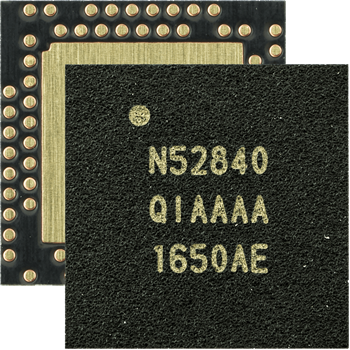
\includegraphics[scale=0.5,angle=0]{nRF52840.png}
	\caption{nRF52840 SoC}
	\label{img:nRF52840}
\end{figure} 


\subsection{Energy Harvesting System (EHS)}\label{subsec:EHS}

Das \textit{EHS} beinhaltet fünf unterschiedlichen Methoden um Energie aus der Umgebung aufzufangen. Diese sind in der folgenden Tabelle mit den wichtigsten Kenndaten aufgefasst. 

\begin{table}[H]
	\centering
	\begin{tabular}{|c|c|l|l|l|}\hline
		\textbf{Quelle} & \textbf{Leistungsdichte} & \textbf{Technologie} & \textbf{Vorteile} & \textbf{Nachteile} \\ \hline
		
		Solar & Innenbereich: 10  $\mu$W/cm2  \newline Aussenbereich: 10 mW/cm2 & Photovoltaic & Hohe Leistungsdichte \newline Ausgereift & Nicht immer verfügbar \newline Benötigt exponierte Oberfläche (nicht Implementierbar) \newline Teuer \\ \hline
		
		Vibration & Mensch: 4 $\mu$W/cm2 \newline Industrie: 100 $\mu$W/cm2 & Piezoelektrisch \newline Elektrostatisch \newline Elektromagnetisch & Implementierbar \newline Hohe Effizienz & Nicht immer verfügbar \\ \hline
		
		
		
	\end{tabular}
	\caption{Lieferobjekte und wichtige Meilensteine}
	\label{tbl:Lieferobjekte}
\end{table} 